\documentclass{beamer}
%
% Choose how your presentation looks.
%
% For more themes, color themes and font themes, see:
% http://deic.uab.es/~iblanes/beamer_gallery/index_by_theme.html
%
\mode<presentation>
{
  \usetheme{default}      % or try Darmstadt, Madrid, Warsaw, ...
  \usecolortheme{beaver} % or try albatross, beaver, crane, ...
  \usefonttheme{default}  % or try serif, structurebold, ...
  \setbeamertemplate{navigation symbols}{}
  \setbeamertemplate{caption}[numbered]
} 

\usepackage[english]{babel}
\usepackage[utf8x]{inputenc}
\usepackage{hyperref}
\hypersetup{
    colorlinks=true,
    linkcolor=blue,
    filecolor=magenta,      
    urlcolor=blue,
}

\title[Presentation]{Presentation}
\author{Andrés Pérez}
\institute{Digital Lutherie\\Master en Música para Experiencias del Entretenimiento\\ENTI-UB}
\date{2019/2020}

\newcommand\blfootnote[1]{%
  \begingroup
  \renewcommand\thefootnote{}\footnote{#1}%
  \addtocounter{footnote}{-1}%
  \endgroup
}

%\AtBeginSection[]
%{
%\begin{frame}{Outline}
%    \tableofcontents[currentsection] 
%\end{frame}
%}

\begin{document}

\begin{frame}
  \titlepage
\end{frame}



%\begin{frame}{Outline}
% \tableofcontents
%\end{frame}

%%%%%%%%%%%%%%%%%%%%%%%%%%%%%%%%%%%%%%%%%%%%%%%%%%
%%%%%%%%%%%%%%%%%%%%%%%%%%%%%%%%%%%%%%%%%%%%%%%%%%
%%%%%%%%%%%%%%%%%%%%%%%%%%%%%%%%%%%%%%%%%%%%%%%%%%
\section{Presentation}
%
%\begin{frame}{Presentation}
%    \textbf{Digital Lutherie}
%    \begin{itemize}
%        \item Digital: related to computers
%        \item Lutherie: musical instrument design and construction
%    \end{itemize}
%\end{frame}

\begin{frame}{About me}
    \begin{itemize}
    \item Education
    \begin{itemize}
        \item Telecommunication Engineer (2011, UPV)
        \item Master in Sound and Music Computing (2014, UPF)
        \item PhD Acoustic Signal Processing (2020, UPF)
    \end{itemize}
    \item Teaching Experience
    \begin{itemize}
        \item Since 2016: Teacher in Audiovisual Systems Engineering, UPF
        \item Since 2018: Teacher at ENTI
        \item Since 2019: Teacher at UOC
    \end{itemize}
    \item Professional Experience
    \begin{itemize}
        \item Research Engineer at Eurecat
    \end{itemize}
        \end{itemize}
\end{frame}


\begin{frame}{About me}
	\begin{figure}[h]
        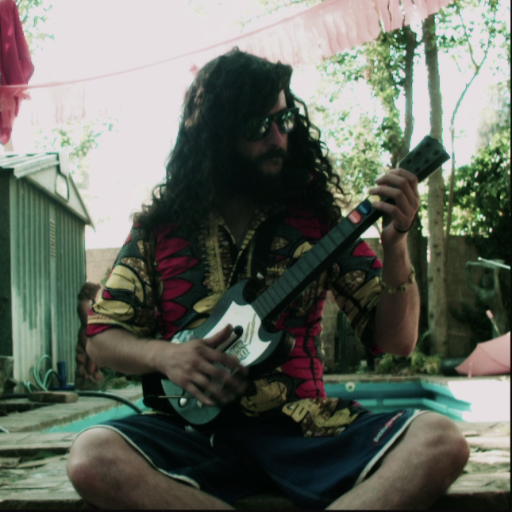
\includegraphics[width=0.5\textwidth]{foto1_vagabundo.png}	
    \end{figure}
\end{frame}

\begin{frame}{About me}
	andres.perez@enti.cat
\end{frame}

\begin{frame}{About you}
	What about you?
\end{frame}

\begin{frame}{About the subject}
	What do you think the subject is about?
\end{frame}

\begin{frame}{About the subject}
    \textbf{Digital Lutherie}
    \begin{itemize}
        \item Digital: related to computers
        \item Lutherie: musical instrument design and construction
    \end{itemize}
\end{frame}

\begin{frame}{About the course}
	Different learning methodologies:
	\begin{itemize}
		\item Theoretical lesson
		\item Practical lesson
		\item Deliverables
	\end{itemize}
\end{frame}

\begin{frame}{About the course}
	Theoretical lessons (7h)
	\begin{itemize}
		\item Introduction
		\item Control Interfaces
		\item Sound synthesis
		\item Communication Protocols
		\item Feedback and interactivity
		\item Design considerations
	\end{itemize}
	\vspace{5mm}
	Mostly during the first half of the course.
\end{frame}

\begin{frame}{About the course}
	Practical lessons (23h)
	\begin{itemize}
		\item Held at the classroom
		\item Guided, partly-supervised tasks
		\item All over the course
	\end{itemize}
\end{frame}

\begin{frame}{About the course}
	Deliverables (45h)
	\begin{itemize}
		\item "Homework", sometimes started at the classroom
		\item Non-supervised task
		\item Approx. one per week
		\item This is your course evaluation!
	\end{itemize}
\end{frame}

\begin{frame}{About the course}
	Evaluation (45h)
	\begin{itemize}
		\item 6 regular tasks, approx 5h per task
		\item 1 final task, approx 15h
		\item Non-presented deliverables will be graded as 0
	\end{itemize}
	\vspace{5mm}
	Final deliverables mark: $\frac{5 x (P1+P2+P3+P4+P5+P6) + (15 x P7)}{45}$\\
	\vspace{5mm}
	Final course mark: $(0.8x\text{Deliverables}) + (0.2x\text{Participation})$
\end{frame}

%\begin{frame}{Introduction}
%    But... what is a musical instrument?\\
%    \vspace{5mm}
%    \textit{    "...a music instrument is any device used to play and to produce any music, transforming in real-time (i.e. by being played) the actions of one or more performers into sound events".\footnote{Jordà, S. (2004). Digital Instruments and Players : Part II – Diversity, Freedom and Control, (January 2004).}}
%\end{frame}


\end{document}
